%%%%%%%%%%%%%%%%%%%%%%%%%%%%%%%%%%%%%%%%%%%%%%%%%%%%%%%%%%%%%%%%%%%%%%
% Overleaf (WriteLaTeX) Example: Molecular Chemistry Presentation
%
% Source: http://www.overleaf.com
%
% In these slides we show how Overleaf can be used with standard
% chemistry packages to easily create professional presentations.
%
% Feel free to distribute this example, but please keep the referral
% to overleaf.com
%
%%%%%%%%%%%%%%%%%%%%%%%%%%%%%%%%%%%%%%%%%%%%%%%%%%%%%%%%%%%%%%%%%%%%%%

\documentclass[xcolor={dvipsnames}]{beamer}

\mode<presentation>
{
  \usetheme{Madrid}       % or try default, Darmstadt, Warsaw, ...
  \usecolortheme{default} % or try albatross, beaver, crane, ...
  \usefonttheme{default}    % or try default, structurebold, ...
  \setbeamertemplate{navigation symbols}{}
  \setbeamertemplate{caption}[numbered]
}

\usepackage[english]{babel}
\usepackage[utf8x]{inputenc}
\usepackage{graphicx}
\usepackage{hyperref}
  \hypersetup{colorlinks=true}
  \hypersetup{urlcolor=blue}
  \hypersetup{linkcolor = .}
\usepackage{xcolor}
\usepackage{siunitx}
  \sisetup{separate-uncertainty = true}
\DeclareSIUnit\barn{b}
\usepackage{physics}
\usepackage[font=small,labelfont=bf]{caption}
\usepackage{subcaption}
\usepackage[en-GB]{datetime2}
\usepackage{overpic}
\usepackage{feynmp}
\DeclareGraphicsRule{*}{mps}{*}{}
\usepackage{scalerel}
\newcommand{\mylbrace}[2]{\vspace{#2pt}\hspace{6pt}\scaleleftright[\dimexpr5pt+#1\dimexpr0.06pt]{\lbrace}{\rule[\dimexpr2pt-#1\dimexpr0.5pt]{-4pt}{#1pt}}{.}}
\newcommand{\myrbrace}[2]{\vspace{#2pt}\scaleleftright[\dimexpr5pt+#1\dimexpr0.06pt]{.}{\rule[\dimexpr2pt-#1\dimexpr0.5pt]{-4pt}{#1pt}}{\rbrace}\hspace{6pt}}

% Trim in percent
\usepackage{adjustbox}

% No "Figure" prefix
\setbeamertemplate{caption}{\raggedright\insertcaption\par}

% Nice decay amplitude diagrams
\usepackage{amsmath,amssymb,tikz-cd}

% Strike out text
\usepackage[normalem]{ulem}

% For figures with text overlay
\usepackage{overpic}

% Arrows
\usepackage{tikz}
\newcommand{\tikzmark}[1]{\tikz[remember picture] \node[coordinate] (#1) {#1};}

% Colourbox with line breaks
\newcommand{\cbox}[2][lime!20]{%
  \colorbox{#1}{\parbox{\dimexpr\linewidth-2\fboxsep}{\strut #2\strut}}%
}

% Vector arrows
\usepackage[pdftex]{pict2e}

% Checkmark symbol
\def\checkmark{\tikz\fill[scale=0.4](0,.35) -- (.25,0) -- (1,.7) -- (.25,.15) -- cycle;}

% Here's where the presentation starts, with the info for the title slide
\title[Heidelberg tracking meeting]{Velo tracking efficiencies in 2025 pre-TS}

\author[Martin Tat]{Martin Tat}
\institute[Heidelberg]{Heidelberg University}
\date{13th May 2026}

\titlegraphic{
\includegraphics[height = 2.3cm]{lhcb.jpg}\hspace{1.0cm}~%
              
\includegraphics[height = 2.3cm]{HeidelbergLogo.pdf}}

\begin{document}

\begin{frame}
  \titlepage
\end{frame}

% These three lines create an automatically generated table of contents.
%\begin{frame}{Outline}
%  \tableofcontents
%\end{frame}

\begin{frame}{Introduction}
  \vspace{0.0cm}
  {\Large Tracking efficiencies presented at A\&S week:}
  \vspace{0.2cm}
  \begin{itemize}
    \setlength\itemsep{1.0em}
    \item{2024 tracking efficiencies are available to analysts \href{https://gitlab.cern.ch/lhcb-rta/tracking-efficiencies-run-3}{here}}
    \begin{itemize}
      \item[-]{Version 0: Smaller MC samples and with only the main systematic}
      \item[-]{Next release: Updated 2D binning scheme, larger MC samples, multiplicity reweighting}
    \end{itemize}
    \item{2025 efficiencies are currently not released}
    \begin{itemize}
      \item[-]{Velo efficiencies had a large discrepancy between data and MC}
      \item[-]{Unusual behaviour: MC significantly underestimates the tracking efficiency}
      \item[-]{Feedback at A\&S week: Check left-right asymmetries and check if M21/M23 are turned off in MC}
    \end{itemize}
  \end{itemize}
\end{frame}

\begin{frame}{Velo left-right asymmetry}
  \vspace{0.0cm}
  \begin{figure}[htb]
    \centering
    \begin{subfigure}{0.4\textwidth}
      \centering
      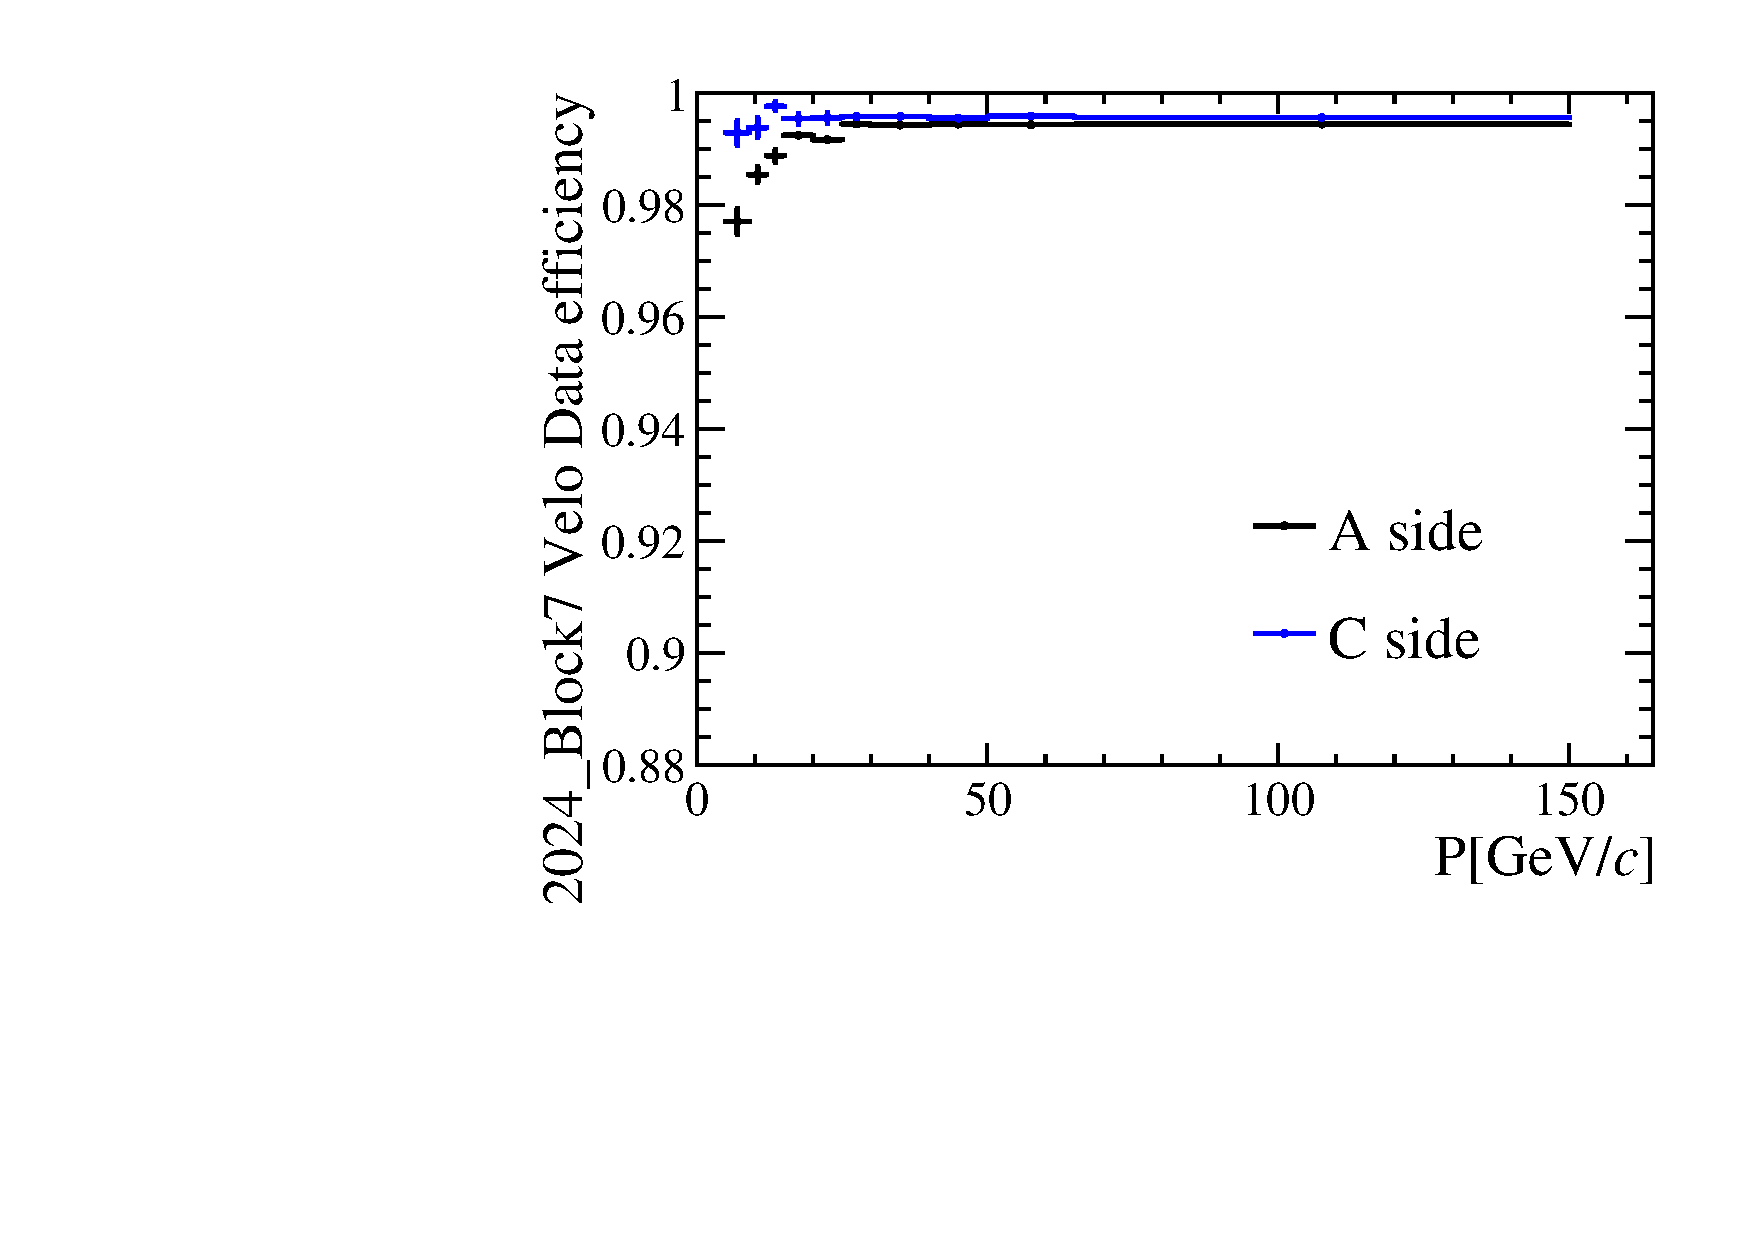
\includegraphics[width=1.0\textwidth]{Plots/trackeff_Data_Downstream_2024_Block7_P_ACside_comparison.pdf}
    \end{subfigure}%
    \begin{subfigure}{0.4\textwidth}
      \centering
      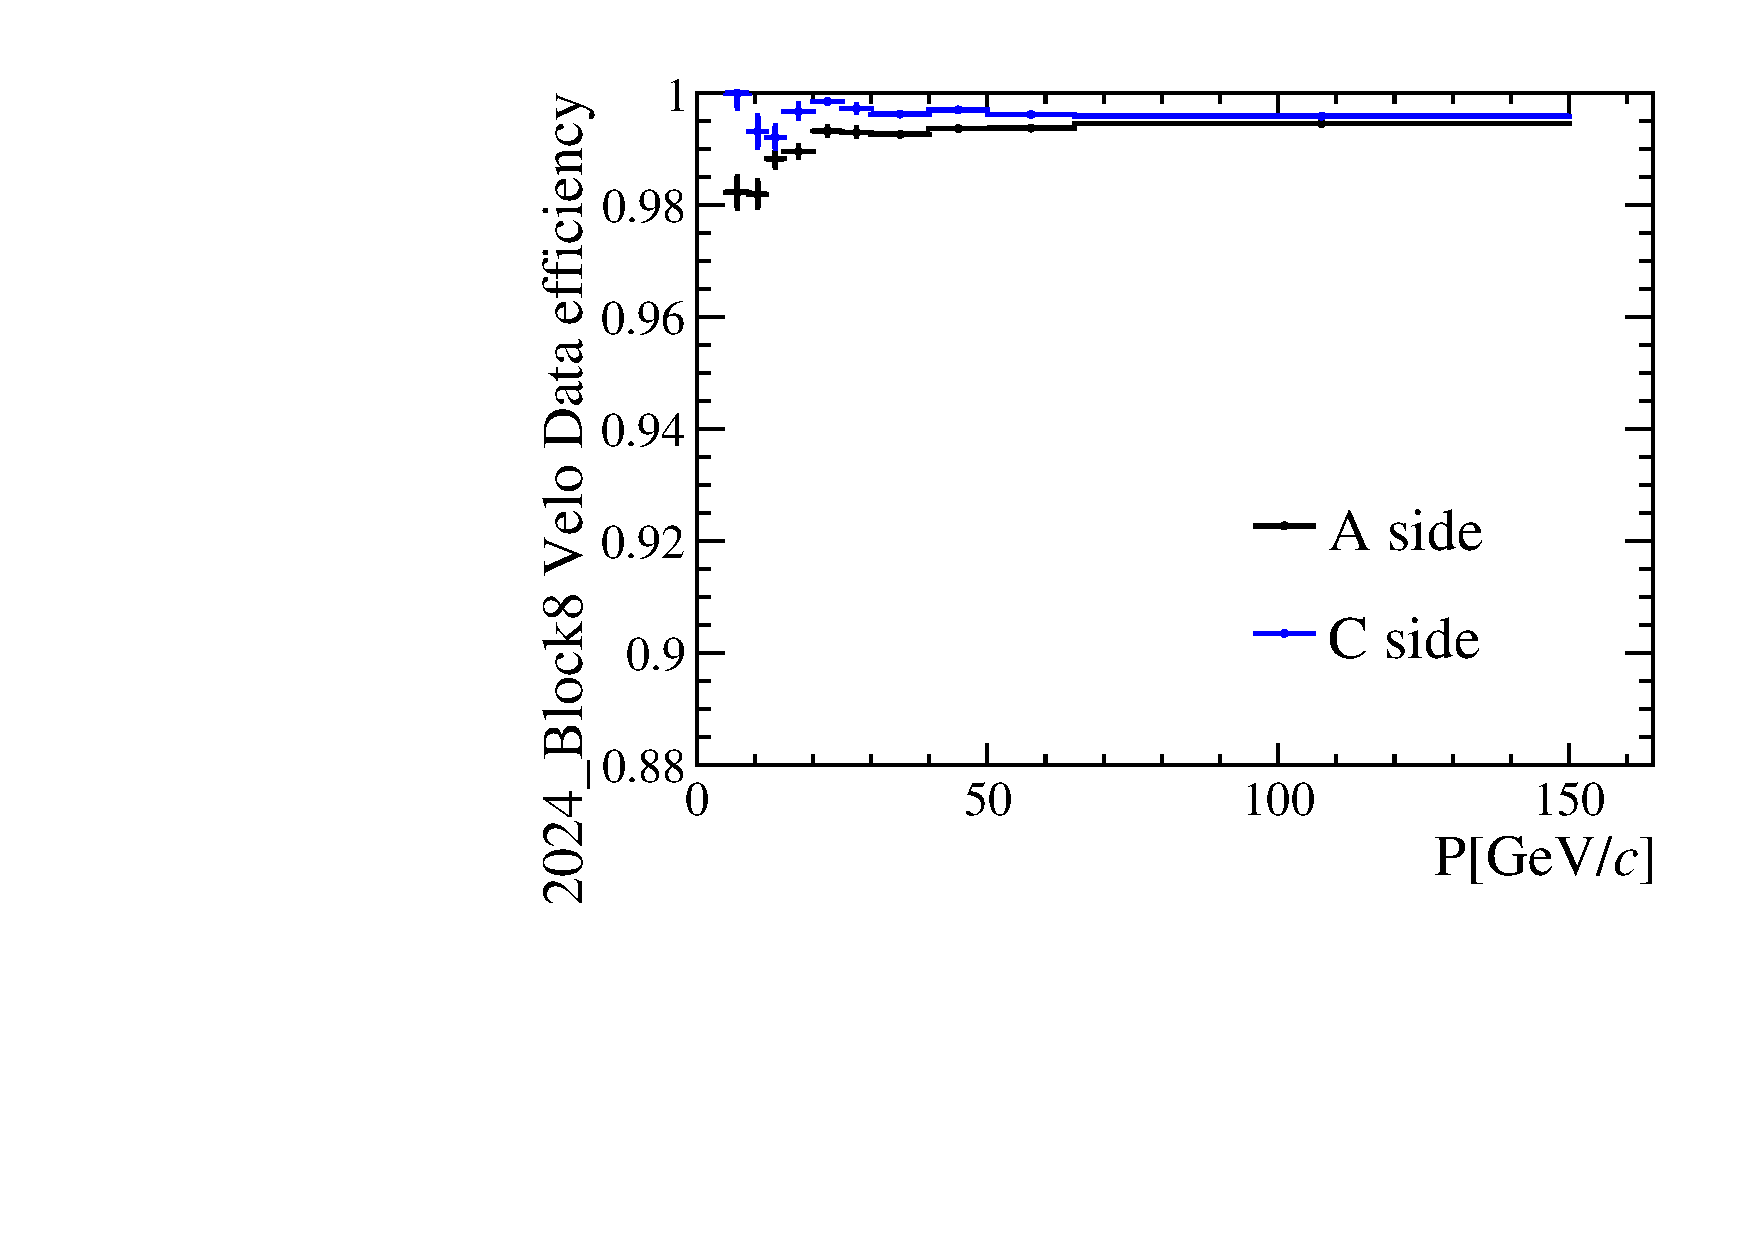
\includegraphics[width=1.0\textwidth]{Plots/trackeff_Data_Downstream_2024_Block8_P_ACside_comparison.pdf}
    \end{subfigure}
    \begin{subfigure}{0.4\textwidth}
      \centering
      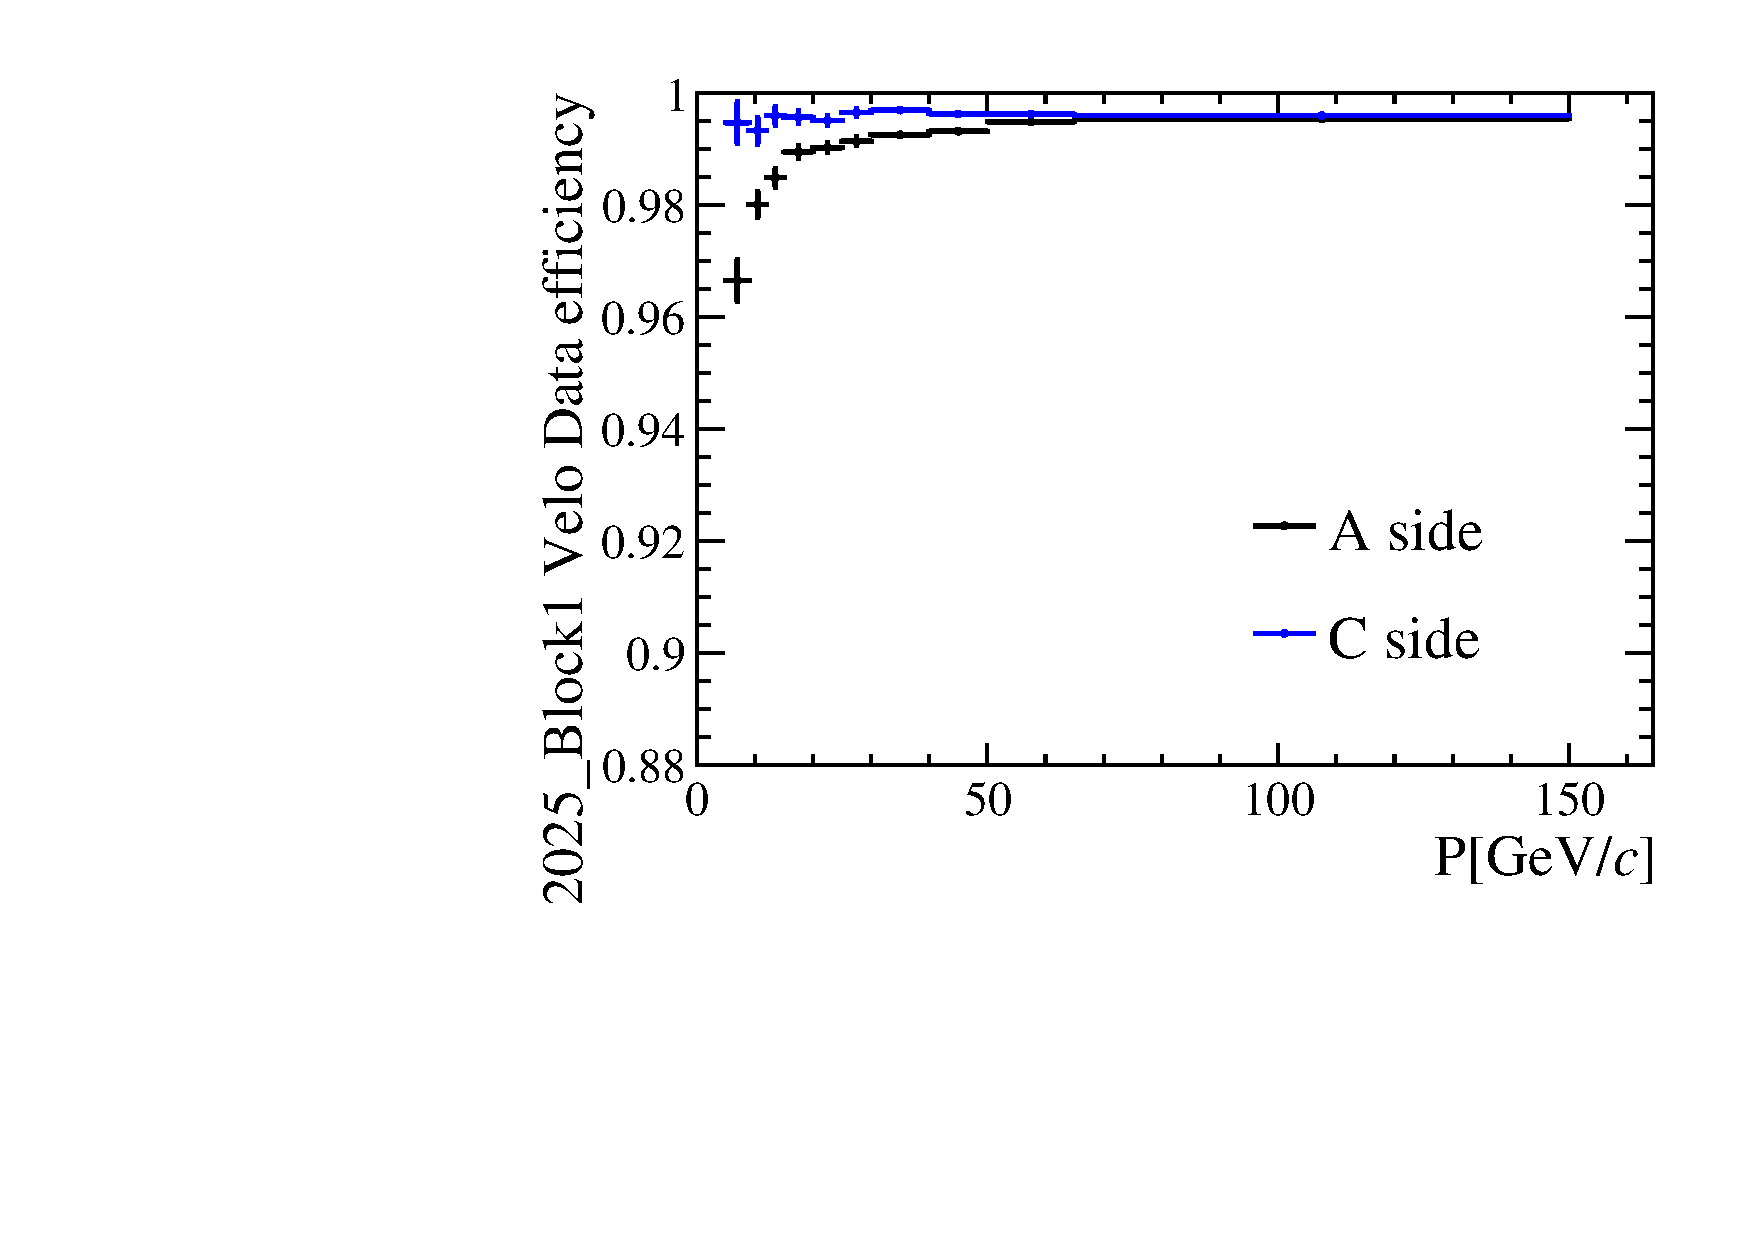
\includegraphics[width=1.0\textwidth]{Plots/trackeff_Data_Downstream_2025_Block1_P_ACside_comparison.pdf}
    \end{subfigure}%
    \begin{subfigure}{0.4\textwidth}
      \centering
      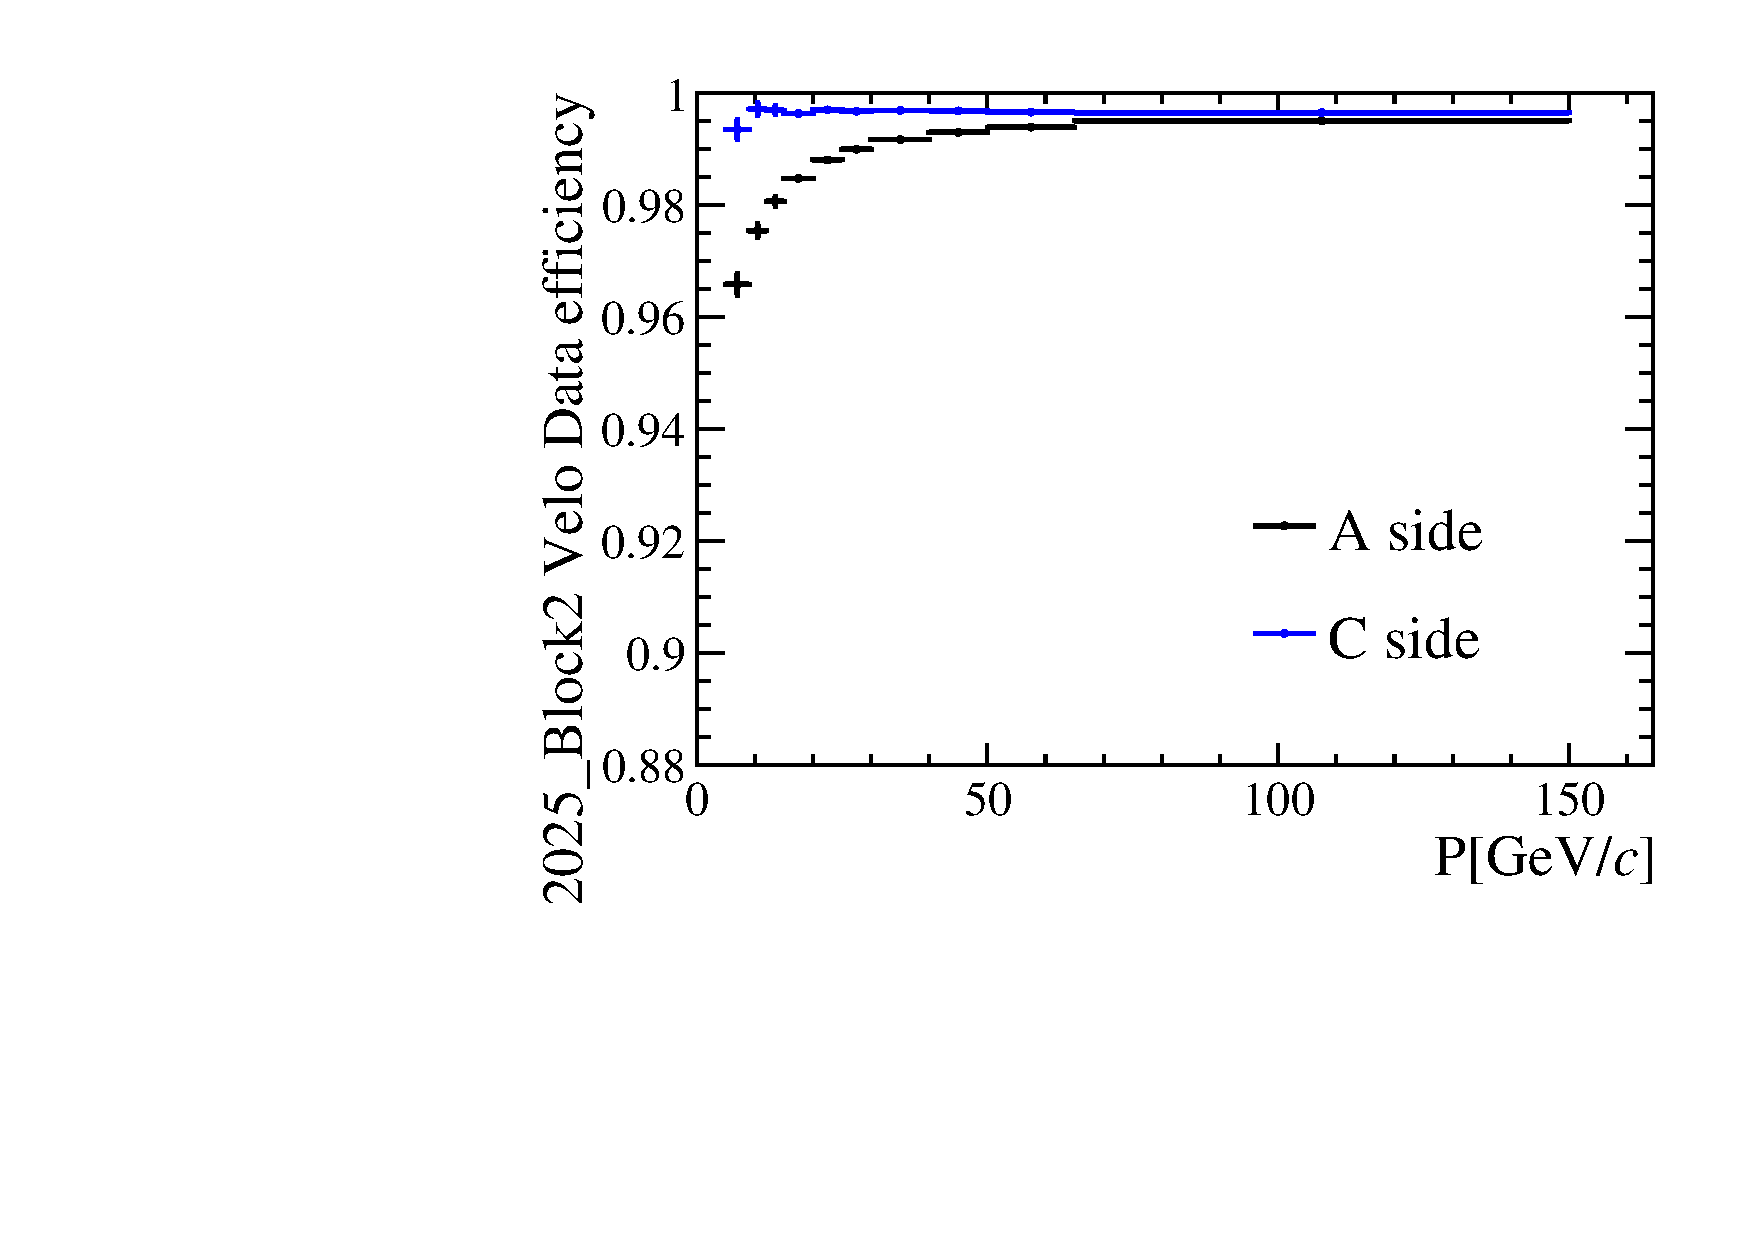
\includegraphics[width=1.0\textwidth]{Plots/trackeff_Data_Downstream_2025_Block2_P_ACside_comparison.pdf}
    \end{subfigure}
  \end{figure}
\end{frame}

\begin{frame}{Velo left-right asymmetry}
  \vspace{0.0cm}
  \begin{figure}[htb]
    \centering
    \begin{subfigure}{0.4\textwidth}
      \centering
      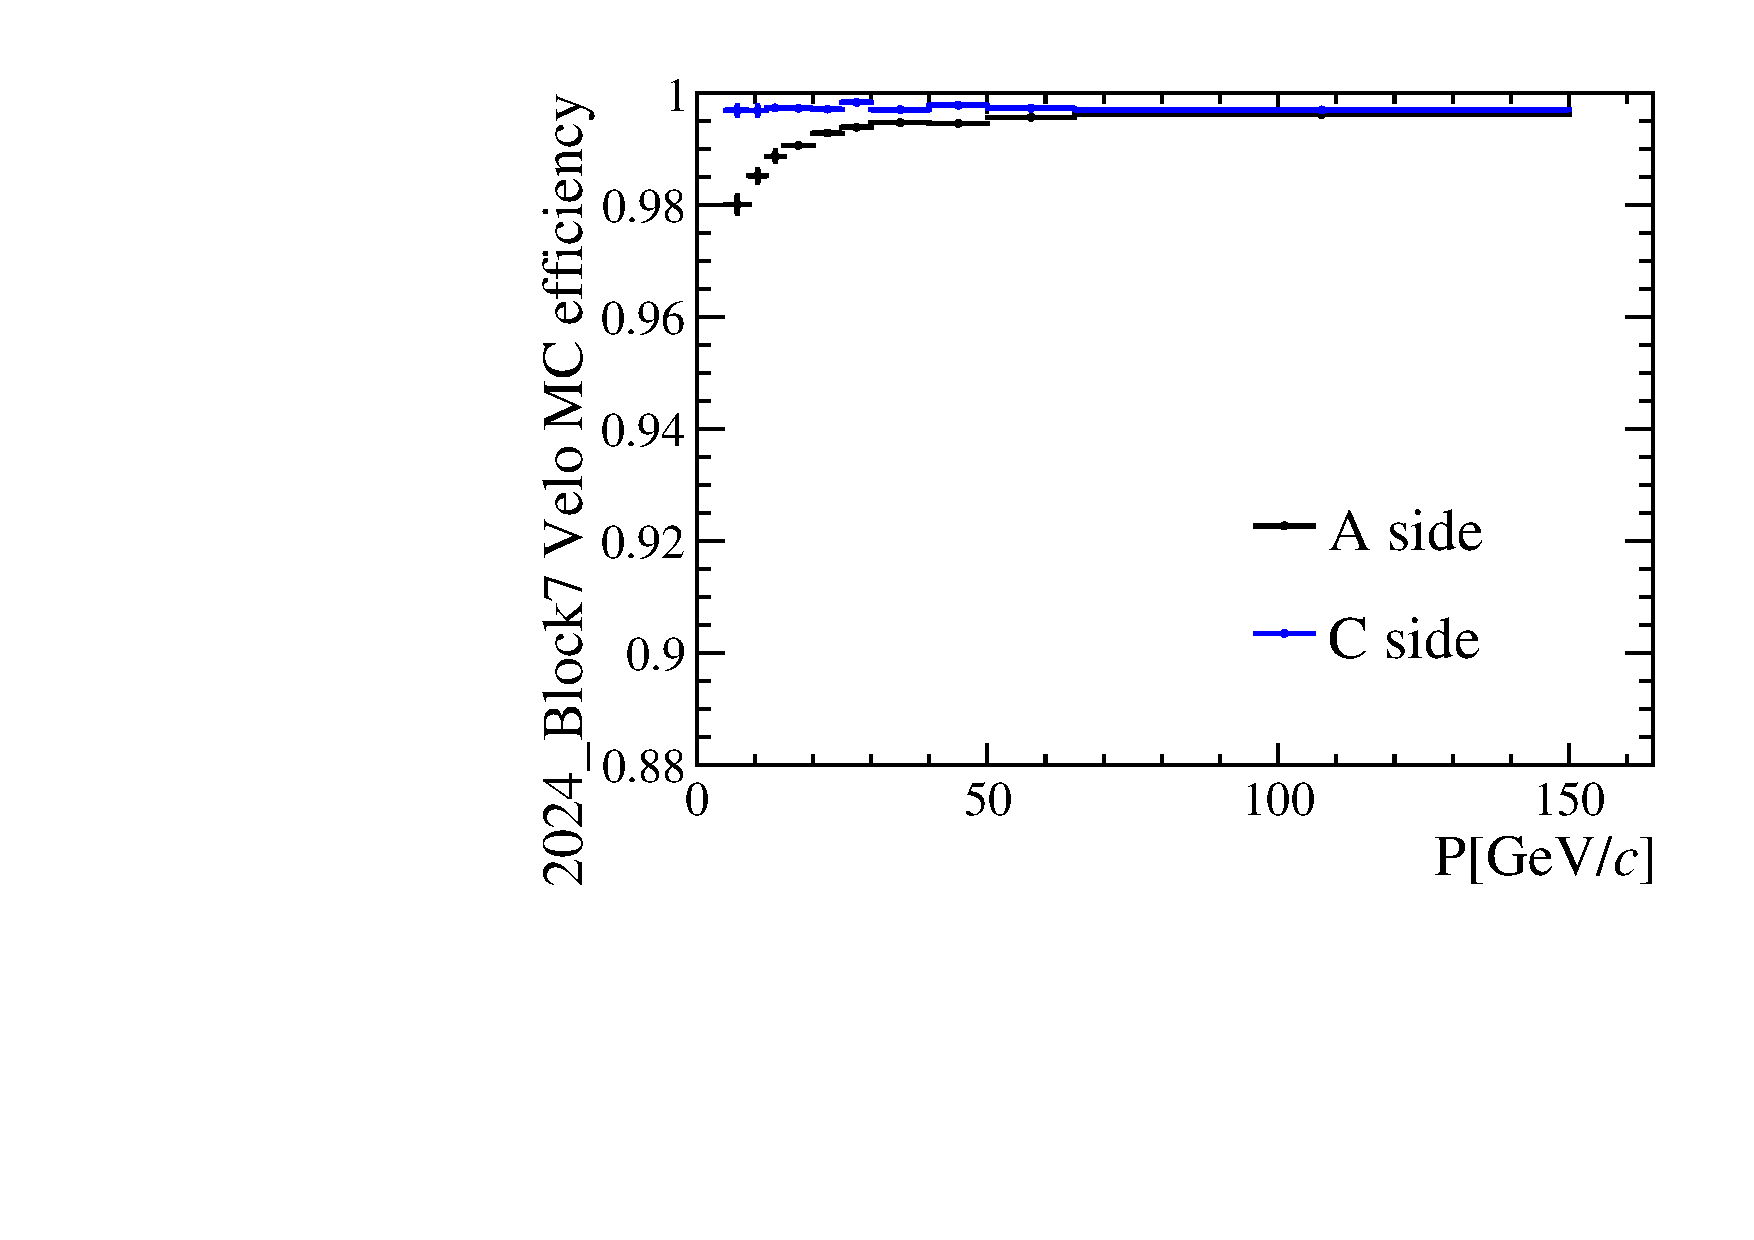
\includegraphics[width=1.0\textwidth]{Plots/trackeff_MC_Downstream_2024_Block7_P_ACside_comparison.pdf}
    \end{subfigure}%
    \begin{subfigure}{0.4\textwidth}
      \centering
      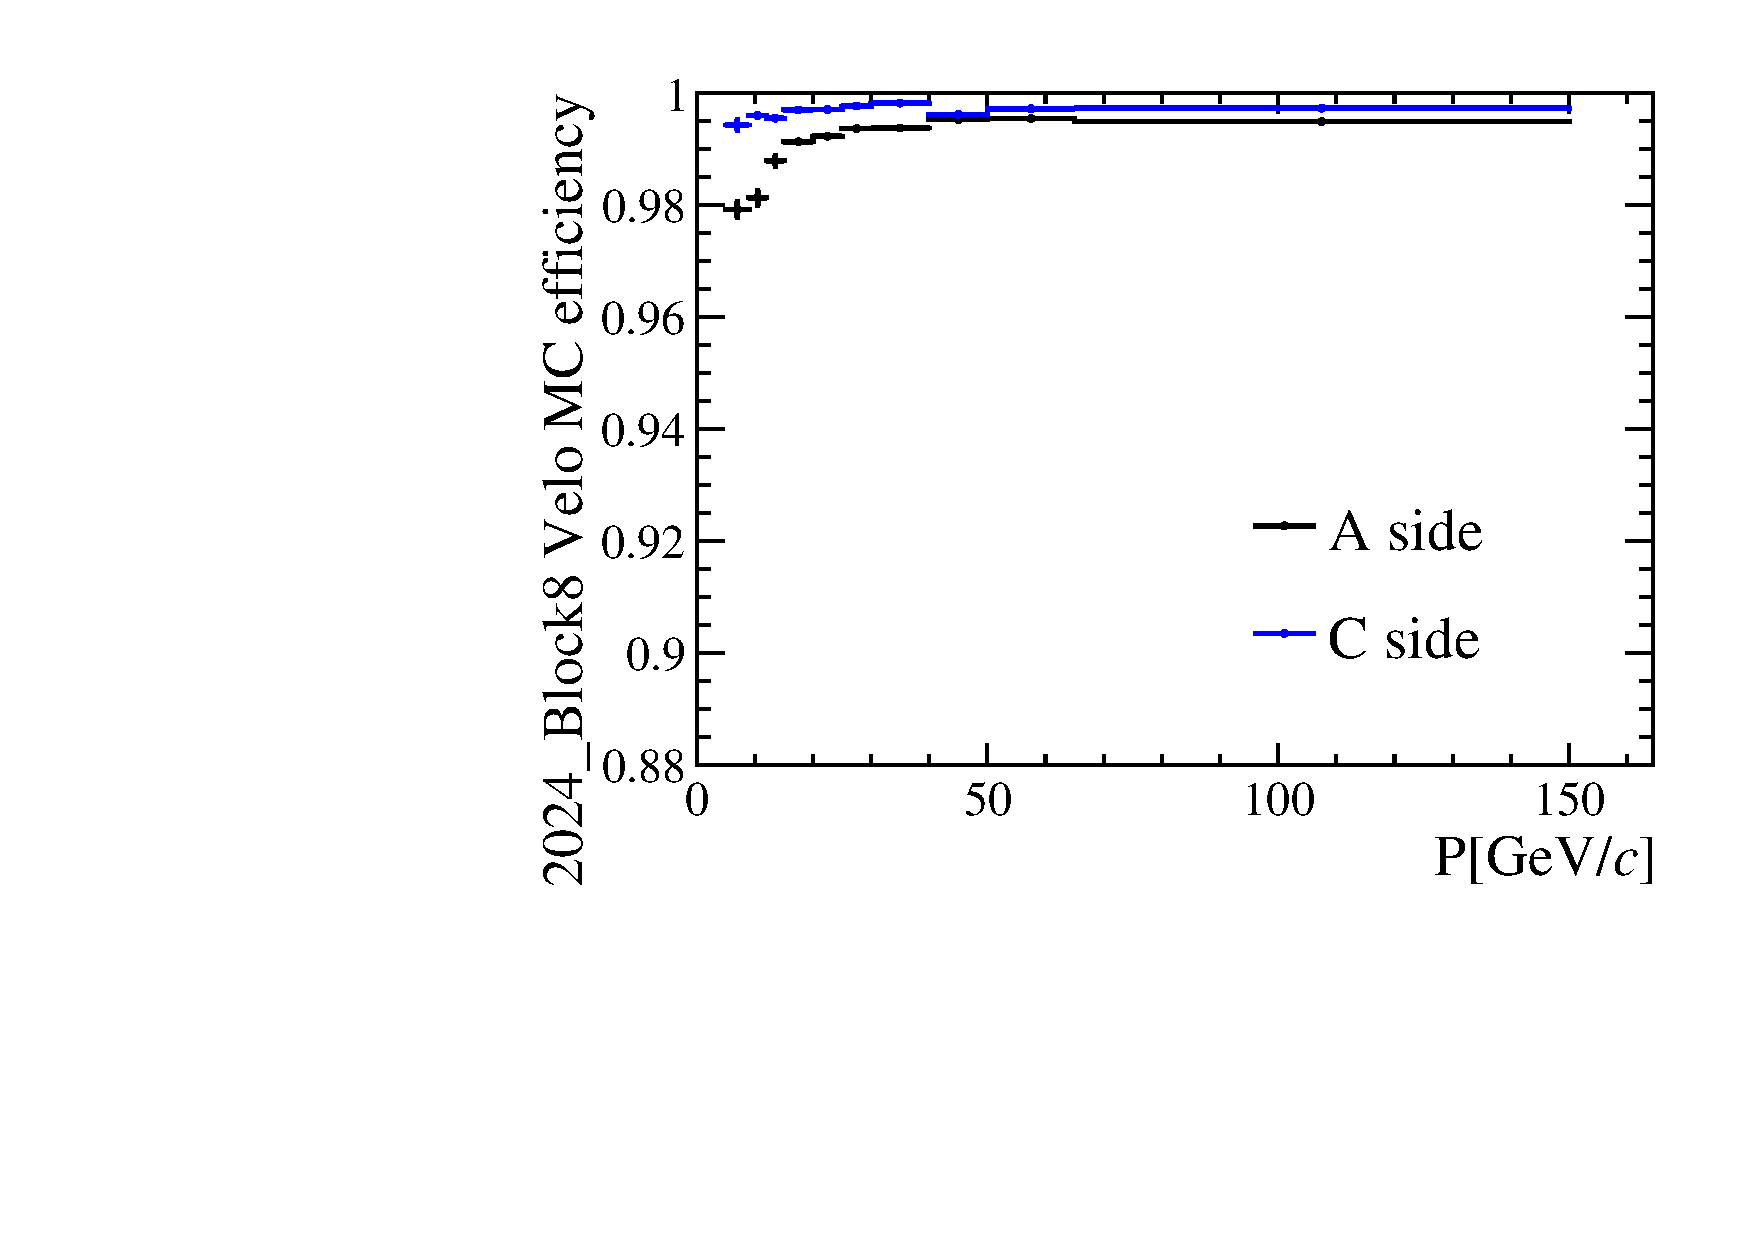
\includegraphics[width=1.0\textwidth]{Plots/trackeff_MC_Downstream_2024_Block8_P_ACside_comparison.pdf}
    \end{subfigure}
    \begin{subfigure}{0.4\textwidth}
      \centering
      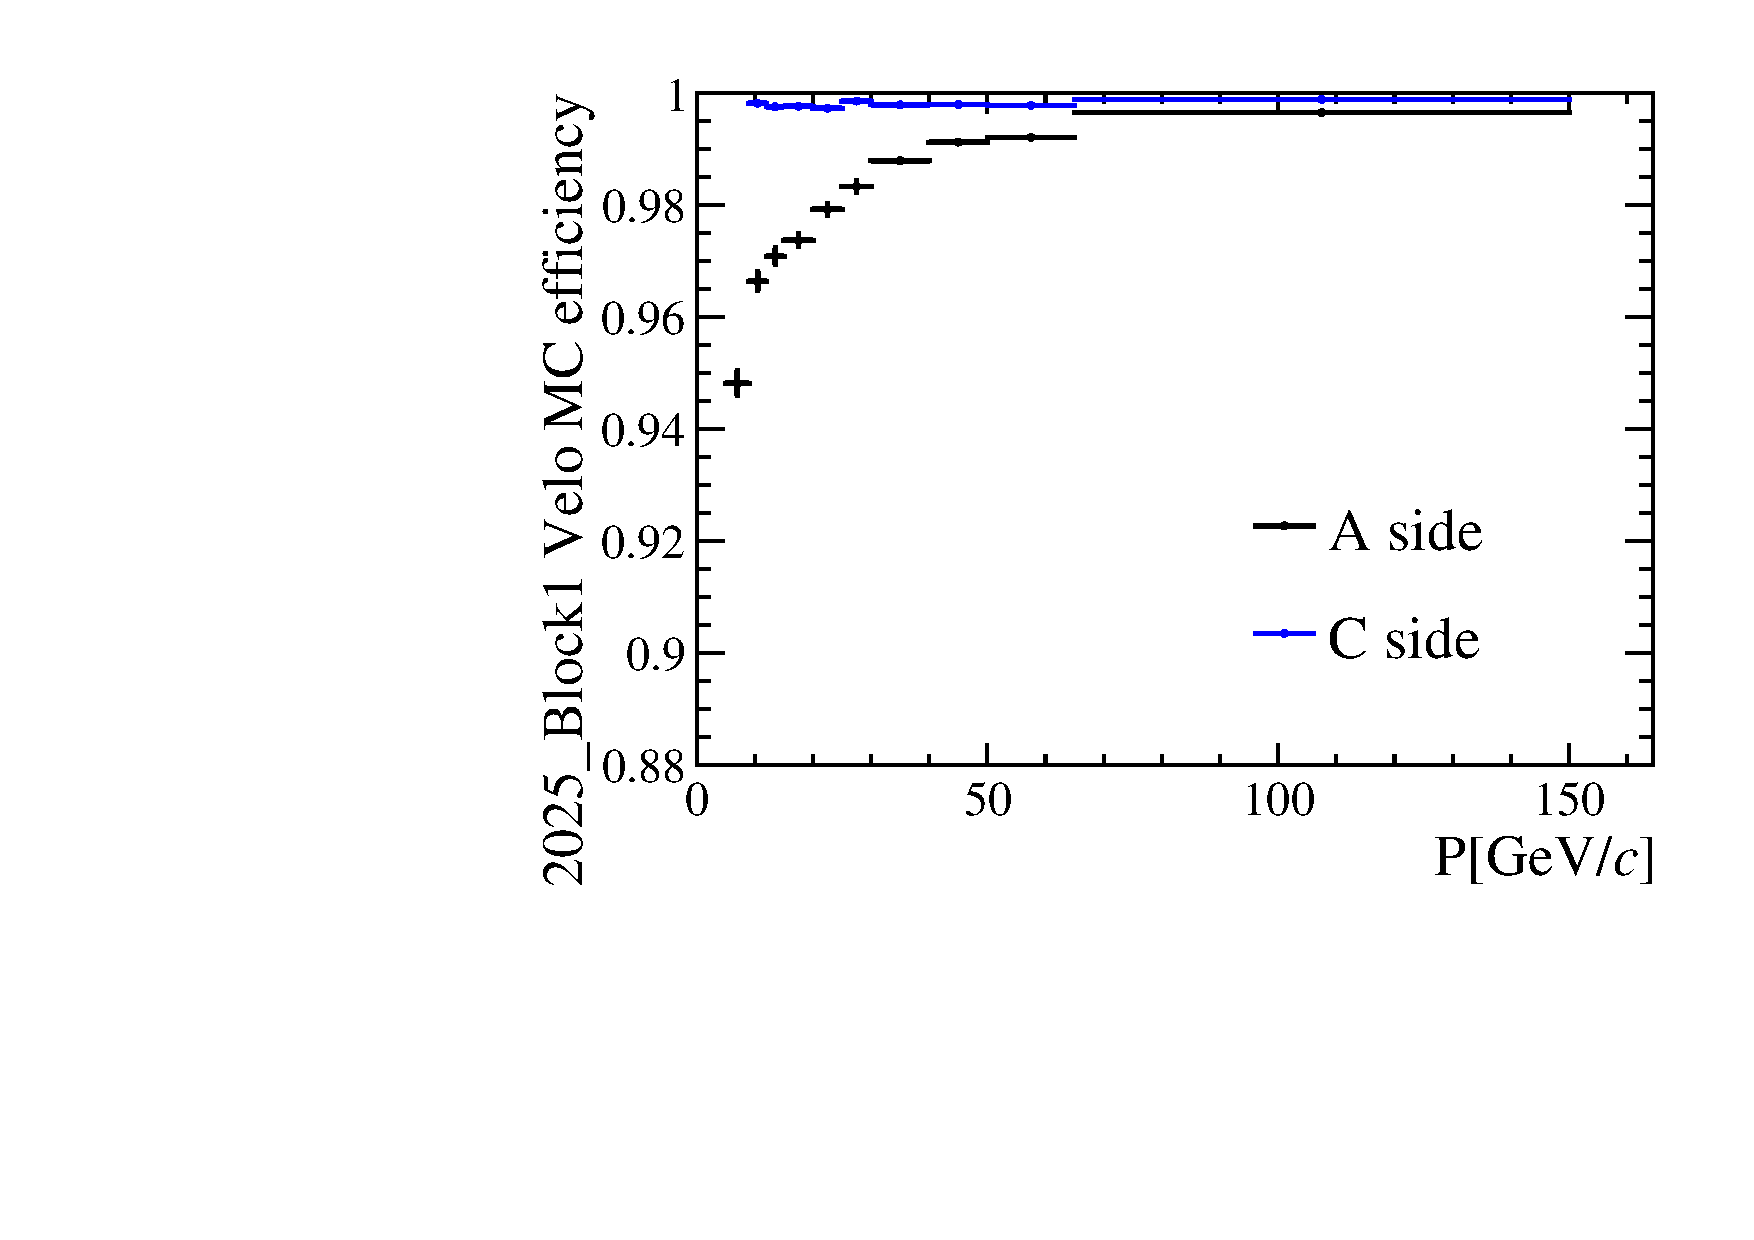
\includegraphics[width=1.0\textwidth]{Plots/trackeff_MC_Downstream_2025_Block1_P_ACside_comparison.pdf}
    \end{subfigure}%
    \begin{subfigure}{0.4\textwidth}
      \centering
      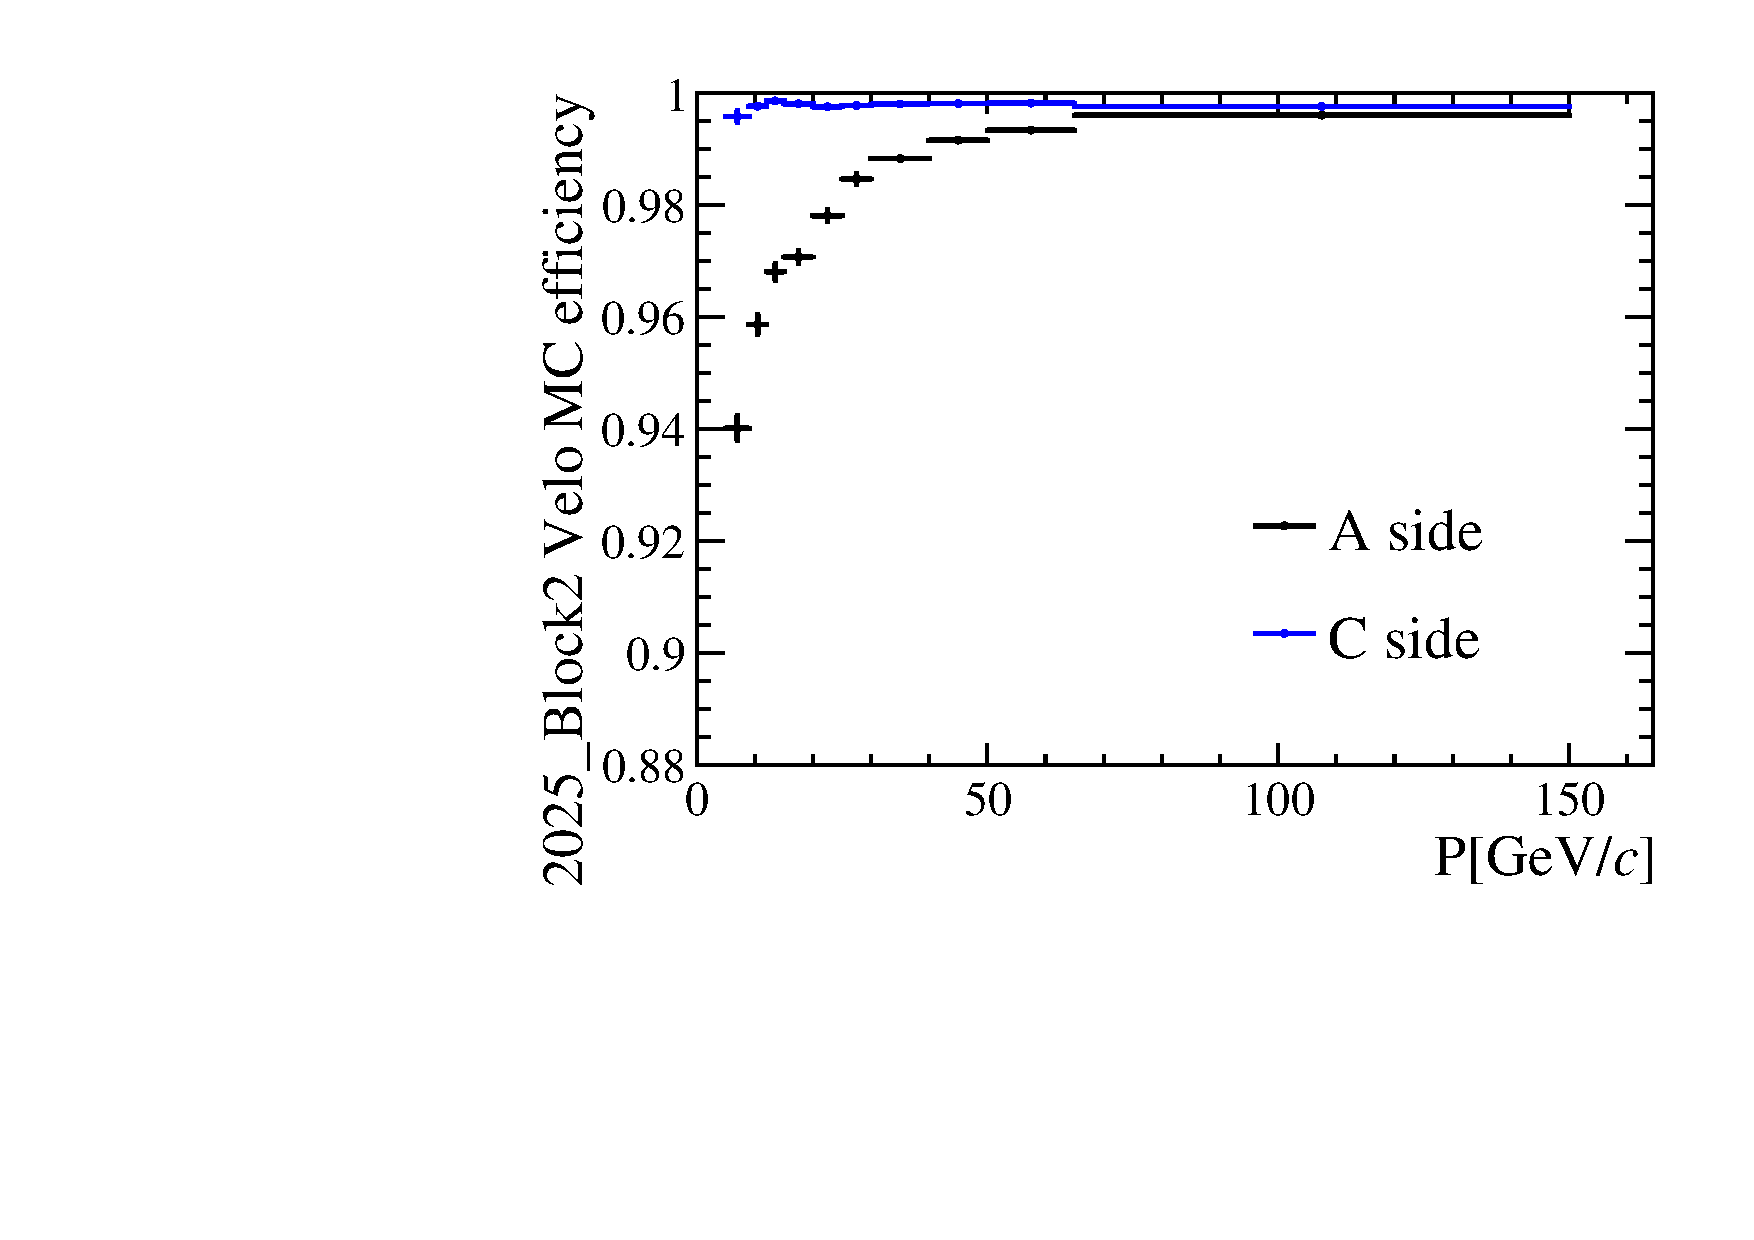
\includegraphics[width=1.0\textwidth]{Plots/trackeff_MC_Downstream_2025_Block2_P_ACside_comparison.pdf}
    \end{subfigure}
  \end{figure}
\end{frame}

\begin{frame}{Velo M21 and M23}
  \vspace{0.0cm}
  {\Large Tracking efficiencies presented at A\&S week:}
  \vspace{0.2cm}
  \begin{itemize}
    \setlength\itemsep{0.5em}
    \item{M21 and M23 sit at $z = \SI{6.875}{\centi\meter}$ and $\SI{9.375}{\centi\meter}$, respectively}
    \item{Each module has 4 sensors}
    \item{M23 in data taking:}
    \begin{itemize}
      \item[-]{2024: All sensors excluded}
      \item[-]{2025 pre-TS: All sensors working}
      \item[-]{2025 post-TS: 2 sensors working}
    \end{itemize}
    \item{M23 in MC:}
    \begin{itemize}
      \item[-]{2024: All sensors excluded}
      \item[-]{2025 pre-TS: All sensors excluded}
      \item[-]{2025 post-TS: 2 sensors working}
    \end{itemize}
    \item{Furthermore, 2 sensors in M21 were not working in 2025 and also turned off in MC}
    \begin{itemize}
      \item[-]{This module is directly in front of M23, so could have significant impact on Velo tracking efficiencies!}
    \end{itemize}
  \end{itemize}
\end{frame}

\begin{frame}{Conclusion and next steps}
  \vspace{0.0cm}
  {\Large We know 2025 pre-TS MC is wrong, what now...?}
  \vspace{0.2cm}
  \begin{itemize}
    \setlength\itemsep{1.0em}
    \item{Simulation group knows and MR with fix was opened a month ago...}
    \item{... but this is low priority and will not be fixed until Sim10i}
    \begin{itemize}
      \item[-]{We're currently on Sim10g!}
    \end{itemize}
    \item{Plan: We need to provide Sim10g corrections to analysts, but be prepared to produce a new set of corrections once Sim10i is available}
    \item{From my side, apart from this data/MC discrepancy, I am ready to release tracking efficiency correction tables for 2025 pre-TS}
    \begin{itemize}
      \item[-]{Need to request MC for the rest of 2025}
      \item[-]{Should in principle have a better data/MC agreement}
    \end{itemize}
  \end{itemize}
\end{frame}

\end{document}
